\chapter*{ВВЕДЕНИЕ}                         % Заголовок
\addcontentsline{toc}{chapter}{ВВЕДЕНИЕ}    % Добавляем его в оглавление

% Заранее ввожу следующие важные определения:

% Метапрограмма - программа на некотором языке программирования, которая в процессе своей работы анализирует, трансформирует или генерирует код на том же или другом языке программирования.
% Просты словами метапрограмма - программа, результатом работы которой является другая программа.

% Метапрограммы это своего рода функции высшего порядка\cite{wiki-hof}, отображения между пространствами программ.

% Метапрограммирование - процесс написания кода метапрограммы.
% \newline
% \vspace{5pt}
% \section*{Актуальность проблемы}
% \section*{}
Язык программирования - основной инструмент любого разработчика. От его эргономики, то насколько легко на нем излагать идеи, напрямую зависит продуктивность разработчика, а также его эмоциональное состояние.

В случае языка Си необходимость линейно упорядочивать определения, вызванная ограничениями по ресурсам вычислительных устройств того времени, когда он был разработан, 
и отсутствие функционала метапрограммирования, понижают его эргономику.

Цель данной работы - повышение эргономики и модернизация языка Си.

% На практике часто встречаются задачи, когда стандартных утилит для работы с языком недостаточно, и приходится писать свои собственные. 
% Например в вашем проекте оптимизац
% Другая цель данного проекта - помочь в разработке подобных утилит, путем предоставления модифицируемого source-to-source компилятора.

Идея состоит в том, чтобы часть функционала компилятора Си, вынести в виде пользовательской библиотеки, с возможность ее модифицирования и доработки. 
Это позволяет разработчику процедурно обрабатывать код, что открывает возможность создания автоматизированных систем по работе с кодом.

Пример такой системы реализован в данной работе с применением синтаксического расширения языка Си, добавляющего \textquote{@ директивы}.

Далее язык Си вместе с автоматизированной системой буду называть просто \textquote{Расширенный Си} (англ. \textquote{Extended C}, сокр. \textquote{EC}). 
% Необходимость такого функционала возникает, когда у разработчика возникает потребность процедурно обрабатывать код

% Си устоявшийся(stable) и стандартизированный язык, 
% поэтому нет проблемы нестабильного API из-за постоянно развивающего языка.%, как например сейчас происходит в Rust.

% Разработчику предлагается использовать данную библиотеку для превращения программного кода в абстрактное синтаксическое дерево - 
% структуру данных, которая может быть обработано процедурно (программным путем).

% Библиотека ec может быть использована отдельно от компилятора ecc для написания своих собственных утилит для работы с языком Си.

В данной работе представлен source-to-source компилятор языка EC - \textquote{Extended C Compiler} (сокр. ecc), представлющий по своей сути слой предобработки исходного кода языка Си, 
с дополнительным функционалом интерпретации директив синтаксического расширения. 




% \section*{Постановка задачи}
Задачами данной выпускной квалификационной работы являются:

\begin{itemize}
    \item Изучение стандартов\cite{c99_std}\cite{c23_std} языка Си
    \item Разработка AST для языка Си по его CFG, написание библиотеки грамматического разбора языка Си
    \item Проектирование синтаксического расширения языка Си
    \item Разработка прототипа компилятора языка EC
    \item Разработка системы макросов для языка EC
\end{itemize}

% \textbf{ecc} является source-to-source компилятором, т.е.компилятором, транслирующих текст программы на одном языке программирования в текст программы 
% на другом (возможно том же самом) языке программирования. 
% В данном случае после разбора текста синтаксическая надстройка на Си интерпретируется, после чего полученное в ходе интерпретации дерево компилируется к тексту языка Си.


% TODO add ref

% \clear
В процессе работы в процессе работы были разобраны следующие источники:

\newcommand{\titlecite}[1]{\citetitle{#1}\cite{#1}}

\titlecite{c23_std}, \titlecite{c99_std} - основные документы, содержащие информацию о языке Си.
В основном использовалась грамматика языка, которая подытожена в Annex A, данных нормативных документов. 
Также использовалась информация о стадиях и порядке трансляции.

\titlecite{crafting_interpreters} - основная книга, использованная в данной работе. 
В ней продемонстрирован метод рекурсивного спуска, описан лексер и парсер для придуманного автором языка Lox.
На основе главы этой книги была написана имплементация хэш-таблицы, использованной в данной работе[\ref{primitives:hashmap}].

\titlecite{hmu} - теория формальных языков, абстрактных вычислительных машин и грамматик. 
Данная книга использовалась как источник математического знания по теме на ранних этапах изучения.

\titlecite{dragon_book} - классическая так называемая \textquote{Книга Дракона}, использовалась на ранних стадиях изучения предметной области для ознакомления с темой.

The Theory of Parsing, Translation, and Compiling (Volume I, II)
\cite{ptc_vI} \cite{ptc_vII} - классические книги по теории компиляции.

\titlecite{monparsing_paper}, \titlecite{ml_syntax_transformation_paper} - статьи про монадические парсеры, рассматривались на ранних стадиях прототипирования парсера.

\titlecite{peg_paper} - оригинальная статья автора PEG грамматики, 
рассматривалась при изучении видов грамматик и парсер-генераторов для грамматик формальных языков.
PEG - Parsing expression grammar, тип аналитической формальной грамматики, является аналогом CFG. 
Однако благодаря свойствам детерминированного оператор выбора в данном формализме в отличие от CFG PEG не может быть неоднозначной, 
т.е. если дерево разбора для грамматики PEG существует, то оно единственное.

\titlecite{parsing_techniques} - при изучении PEG грамматики была рассмотрена глава 15.7 \textquote{Recognition Systems} данной книги.

Были рассмотрены следующие источники по теме \textquote{Разбор выражений и приоритет операций}:
% \subsection*{Разбор выражений и приоритет операций}

% \caption{pratt}
% \label{litover:pratt} \mbox{} \\
\titlecite{tdop_pratt_paper} - оригинальная статья автора парсера Пратта, использовалась для ознакомления с темой.

\titlecite{matklad_pratt_parsers} - из этой статьи позаимствована идея конкретной имплементация парсера Пратта.

\titlecite{cppref_op_prec} - справка по языку Си: приоритет операций, использовалась при построении таблицы[\ref{extras:c_defs}] приоритетов операций.

\titlecite{pest_op_pratt} - парсер Пратта в фреймворке pest.

При разработке парсера были рассмотрены синтаксические деревья и методы грамматического разбора в других языках:

В языке Rust абстрактное синтаксическое дерево\cite{rust-ast} выполнено средствами богатой системы типов Rust, 
такими как энумерации(\verb|enum|), которые в Rust могут выполнять функцию помеченных объединений(tagged unions).
Функционал, доступный под ключевым словом \verb|match|, проверяет, чтобы все под-элементы данного элемента AST были обработаны,
что значительно снижает кол-во ошибок при работе с AST. В данной работе за неимением подобных проверок в Си используются 
функции \textquote{заглушки} \verb|unreachable| и \verb|unimplemented|, рассмотренные далее[\ref{primitives}].

Был рассмотрен парсер Rust\cite{rustc-parser}.
Структура, полученная в ходе лексического разбора кода Rust является вложенной, поэтому в парсере используется стек для итерации по данной структуре.
В данной работе я отказался от использования стека и решил уплощить структуру.


Был рассмотрен язык Odin. Была рассмотрена часть его стандартной библиотеки, отвечающая за его синтаксический разбор и анализ\cite{odin-parser}.
Стандартная библиотека языка Odin служила хорошим примером при разработке библиотеки примитивов[\ref{extras:c-core}]

Было рассмотрено синтаксическое дерево языка Python\cite{python-ast} и интерфейс позволяющий работать с ним. 
Python использовался для изучения AST структуры на этапе изучения предметной области.


Была рассмотрена система генерации \verb|go generate| языка Go, описанная в статье \titlecite{go-gen}.
Данная система рассматривалась совместно с модулями AST\cite{go-ast} и грамматического разбора\cite{go-parser} языка Go.
Следующая статья содержит множество полезных примеров использования данной системы: \titlecite{go-tool-guide}.

Был рассмотрен язык Julia, система метапрограммирования\cite{julia-meta}, 
синтаксически похожая на систему выполненную в данном проекте, подробнее далее[\ref{langcmp:julia}]. 

Был рассмотрен язык Zig и его \verb|comptime| функционал\cite{zig-comptime}.
На основе примеров приведенных в стандартной библиотеке языка Zig были разработаны интерфейс аллокатора[\ref{primitives:allocator}] и виртуальные таблицы для динамических интерфейсов.









% \paragraph*{Актуальность темы.}


% \paragraph*{Цель работы.}

% \paragraph*{Задачи работы.}

% \paragraph*{Научная новизна работы.}

% \paragraph*{Теоретическая и практическая значимость работы.}

% \paragraph*{Положения выносимые на защиту.}
% \begin{enumerate}
%     \item \statementOneRU
%     \item \statementTwoRU 
% \end{enumerate}

% \paragraph*{Апробация работы.}

% \paragraph*{Достоверность научных достижений.}

% \paragraph*{Внедрение результатов работы.}

% \paragraph*{Публикации.} Список всех публикаций автора по теме диссертации:
% \begin{refsection}[biblio/own.bib]
% \nocite{*}
% \printbibliography[
%     keyword=own,
%     %title={Список всех публикаций автора по теме диссертации}, 
%     %heading=subbibliography,
%     heading=none,
%     resetnumbers=true
% ]
% \end{refsection}



% \paragraph*{Структура и объем диссертации. }
% Диссертация состоит из~введения,
% \formbytotal{totalchapter}{глав}{ы}{}{},
% заключения и
% \formbytotal{totalappendix}{приложен}{ия}{ий}{}.
% %% на случай ошибок оставляю исходный кусок на месте, закомментированным
% %Полный объём диссертации составляет  \ref*{TotPages}~страницу
% %с~\totalfigures{}~рисунками и~\totaltables{}~таблицами. Список литературы
% %содержит \total{citenum}~наименований.
% %
% Полный объём диссертации составляет
% \formbytotal{TotPages}{страниц}{у}{ы}{}, включая
% \formbytotal{totalcount@figure}{рисун}{ок}{ка}{ков} и
% \formbytotal{totalcount@table}{таблиц}{у}{ы}{}.
% Список литературы содержит
% \formbytotal{citenum}{наименован}{ие}{ия}{ий}.


% \begin{figure}
%     \centering
%     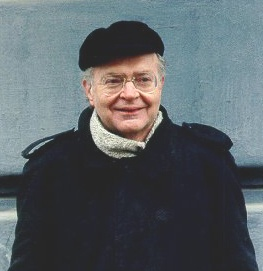
\includegraphics[width=0.6\linewidth]{images/knuth}
%     \caption{Knuth}
%     \label{fig:my_label}
% \end{figure}